\documentclass[a4paper,12pt]{article}

% Sprach- und Zeichensatz
\usepackage[ngerman]{babel}
\usepackage[utf8]{inputenc}
\usepackage[T1]{fontenc}

% Seitenlayout und Typografie
\usepackage{geometry}
\geometry{margin=2.5cm}
\usepackage{setspace}
\onehalfspacing
\usepackage{lmodern}

% Aufzählungen
\usepackage{enumitem}

% Grafiken
\usepackage{graphicx}

\title{Aufgabenblatt 0: Positives Beispiel einer Informationsvisualisierung}
\author{Tim Lukas}
\date{\today}

\begin{document}

\maketitle

\section{Einleitung}
Dieses Dokument bewertet eine Beispielgrafik, die als positives Beispiel für eine gelungene Informationsvisualisierung dient.  
Ziel ist es, die wesentlichen Merkmale der Darstellung zu analysieren und ihre Wirkung zu bewerten.

\section{Beispielgrafik}
Abbildung~\ref{fig:beispiel} zeigt eine lokale Grafik, die Marktanteile im Smartphone-Markt visualisiert.

\begin{figure}[h!]
    \centering
    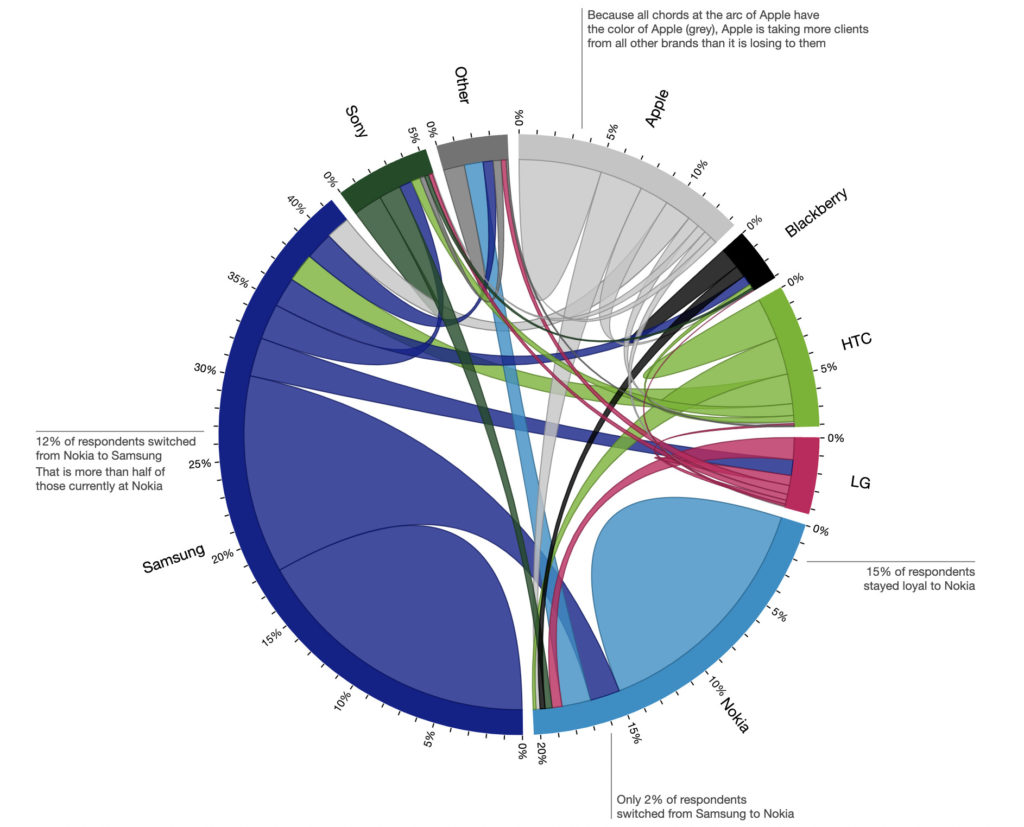
\includegraphics[width=0.7\textwidth]{Visualisierungsbeispiel_tim_lukas.JPG}
    \caption{Visualisierung der Marktanteile im Smartphone-Markt.}
    \label{fig:beispiel}
\end{figure}

\section{Analyse der Grafik}
Die gezeigte Abbildung stellt ein sogenanntes \textit{Chord-Diagramm} dar, welches die Wechselbeziehungen zwischen verschiedenen Smartphone-Marken visualisiert. 
Dabei werden sowohl Abwanderungs- als auch Loyalitätsströme der Befragten gleichzeitig dargestellt. 
Im Folgenden werden zunächst die positiven Aspekte der Darstellung hervorgehoben, bevor auf mögliche Schwächen eingegangen wird.

\subsection{Positive Aspekte}
Die Grafik weist mehrere Merkmale auf, die eine gelungene Informationsvisualisierung auszeichnen:

\begin{itemize}[label=--]
    \item \textbf{Übersichtliche Darstellung komplexer Beziehungen:} 
    Das Chord-Diagramm ermöglicht es, Wechselbewegungen zwischen Marken in einer kompakten, zusammenhängenden Struktur zu visualisieren. 
    Dadurch wird ein umfassender Überblick über Marktbewegungen geschaffen.
    
    \item \textbf{Konsistente Farbgestaltung:} 
    Jede Marke ist mit einer eindeutigen Farbe versehen, wodurch Zu- und Abflüsse intuitiv zugeordnet werden können. 
    Die Farbverläufe machen die Richtung der Wechsel klar erkennbar.
    
    \item \textbf{Hoher Informationsgehalt auf engem Raum:} 
    Das Diagramm kombiniert Mengenangaben, Prozentwerte und Markenbeziehungen in einer einzigen Darstellung, ohne überladen zu wirken.
    
    \item \textbf{Ergänzende Textkommentare:} 
    Kurze erklärende Texte an den relevanten Stellen (z.\,B. Wechsel von Nokia zu Samsung) erleichtern das Verständnis und betonen zentrale Erkenntnisse.
    
    \item \textbf{Visuelle Balance und Ästhetik:} 
    Trotz der Vielzahl an Verbindungen bleibt die Grafik visuell ausgewogen. 
    Der kreisförmige Aufbau sorgt für eine harmonische, gut lesbare Gesamtstruktur.
\end{itemize}

\subsection{Negative Aspekte}
Neben den genannten Stärken zeigt die Grafik auch einige Schwächen und mögliche Verbesserungspotenziale:

\begin{itemize}[label=--]
    \item \textbf{Hohe kognitive Belastung:} 
    Für ungeübte Betrachter ist die Interpretation des Diagramms anspruchsvoll, insbesondere das Nachvollziehen der Verbindungen und Flussrichtungen.
    
    \item \textbf{Teilweise eingeschränkte Lesbarkeit:} 
    Einige Beschriftungen und Prozentangaben sind klein oder überlappen sich, was die Zugänglichkeit erschwert.
    
    \item \textbf{Fehlende Legende:} 
    Eine kurze Legende oder Erläuterung zur Farbcodierung und Richtung der Flüsse würde das Verständnis deutlich erleichtern.
    
    \item \textbf{Keine zeitliche Dimension:} 
    Die Grafik zeigt einen statischen Zustand. 
    Eine Erweiterung um zeitliche Entwicklungen oder Veränderungen könnte zusätzliche analytische Tiefe bieten.
\end{itemize}

\subsection{Fazit}
Zusammenfassend ist die Grafik ein gutes Beispiel für eine anspruchsvolle, aber informative Visualisierung. 
Sie besitzt einen hohen Informationsgehalt, der dennoch nachvollziehbar abgebildet wird.
Die Grafik kann bei der ersten Betrachtung überwältigend wirken, setzt man sich jedoch etwas intensiver mit ihr auseinander, können die vermittelten Informationen trotz 
der hohen Komplexität gut nachvollzogen werden.

\end{document}
